% FGCS
\documentclass[final,5p,times,twocolumn]{elsarticle}

\usepackage[english]{babel}
\usepackage[utf8]{inputenc}
\usepackage{amsmath}
\usepackage{graphicx}
\usepackage[colorinlistoftodos]{todonotes}
\usepackage{hyperref}
\usepackage{soul}
\usepackage{algorithm}
\usepackage{algorithmic}
\usepackage{makeidx} 
\usepackage[section]{placeins}
\usepackage{float}
\usepackage{listings, multicol}

\usepackage{color}
\definecolor{mygray}{rgb}{0.5,0.5,0.5}

\lstset{ 
  showspaces=false,     
  }


% Commands
\newcommand{\comment}[2][inline]{\todo[color=yellow!30,#1]{\small\sf #2}}
\newcommand{\note}[2][inline]{\color{red} [TODO]: #2\color{black}}

\journal{Future Generation Computer Systems}

\begin{document}
\begin{frontmatter}

% Title
\title{A Semantic-Based Approach to Attain Reproducibility of Computational Environments in Scientific Workflows: A Case Study}

% Authors and Institutions
\author[upm]{Idafen Santana-Perez\corref{cor1}}
\ead{isantana@fi.upm.es}

\author[isi]{Rafael Ferreira da Silva}
\ead{rafsilva@isi.edu}

\author[isi]{Mats Rynge}
\ead{rynge@isi.edu}

\author[isi]{Ewa Deelman}
\ead{deelman@isi.edu}

\author[upm]{Mar\'ia~S.~P\'erez-Hern\'andez}
\ead{mperez@fi.upm.es}

\author[upm]{Oscar Corcho}
\ead{ocorcho@fi.upm.es}

\cortext[cor1]{Corresponding address: Ontology Engineering Group (OEG), Laboratorio de Inteligencia Artificial, Facultad de Inform\'atica, Universidad Polit\'ecnica de Madrid, Avda. Montepr\'incipe, s/n, Boadilla del Monte, 28660, Spain}

\address[upm]{Ontology Engineering Group, Universidad Polit\'ecnica de Madrid, Madrid, Spain }
\address[isi]{University of Southern California, Information Sciences Institute, Marina del Rey, CA, USA}


% Abstract
\begin{abstract}
Reproducible research in scientific workflows is often addressed by tracking the provenance of the produced results. While this approach allows inspecting intermediate and final results, improves understanding, and permits replaying a workflow execution, it does not ensure that the computational environment is available for subsequent executions to reproduce the experiment. In this work, we propose describing the resources involved in the execution of an experiment using a set of semantic vocabularies, so as to conserve the computational environment. We define a process for documenting the workflow application, management system, and their dependencies based on 4 domain ontologies. We then conduct an experimental evaluation using a real workflow application on an academic and a public Cloud platform. Results show that our approach can reproduce an equivalent execution environment of a predefined virtual machine image on both computing platforms.
\end{abstract}

\begin{keyword}
Semantic Metadata \sep Scientific Workflow \sep Reproducibility
\end{keyword}


\end{frontmatter}


% Sections
\section{Introduction}

Reproducibility of results of scientific experiments is a cornerstone \rev{of the scientific 
method}. Therefore, the scientific community has been encouraging researchers 
to publish their contributions in a verifiable and understandable 
way~\cite{YaleRoundtable09, James-XSEDE-2014}. In computational science, 
or \emph{in-silico} science, reproducibility often requires that researchers make 
code and data publicly available so that the data can be analyzed in a similar 
manner as in the original work described in the publication. Code must be \rev{made } available, 
and data must be accessible in a readable format~\cite{bookReproducibility}. 

Scientific workflows are a useful representation for managing the execution of large-scale 
computations. Many scientists now formulate their computational problems as scientific 
workflows running on distributed computing infrastructures such as campus Clusters, 
Clouds, and Grids~\cite{workflowBook}. Researchers in bioinformatics have 
embraced workflows for a whole range of analyses, including protein folding~\cite{craddock2006science}, 
DNA and RNA sequencing~\cite{blankenberg2010galaxy, giardine2005galaxy, kepler-clotho}, 
and disease-related research~\cite{fisher2009systematic, gaizauskas2004}, among others.
The workflow representation not only facilitates the creation and management of the 
computation but also builds a foundation upon which results can be validated and 
shared. 

\rev{Much research has focused } on studying the reproducibility of scientific results 
in life sciences. Some studies clearly show the difficulties when trying to replicate 
experimental results in biology~\cite{Ioannidis2009}. The \emph{Reproducibility 
Project: Cancer Biology}~\cite{ErringtonCancerRerpoducibility} is an active project 
aiming to independently reproduce the experimental results of 50 high-impact cancer 
biology studies, evaluating the degree of reproducibility of those results and the main 
issues related to them.


Since workflows formally describe the sequence of computational and data 
management tasks, it is easy to trace the origin of the data produced. Many workflow 
systems capture provenance at runtime, what provides the lineage of data products 
and as such underpins scientific \rev{understanding and } data reuse by providing the basis on which 
trust and understanding are built. A scientist would be able to look at the workflow and 
provenance data, retrace the steps, and arrive at the same data products. 
However, this information is not sufficient for achieving full reproducibility.

%\note{Idafen, better introduce here concepts such as: Reproducibility, replicability, conservation,...}

Reproducibility, replicability, and repeatability are often used as synonyms. Even when they
\rev{pursue } similar goals, there are several differences between them~\cite{Drummond2011}. In this work we consider them
as separated concepts. While replicability can be defined as a
strict recreation of the original experiment, using the same method, data and equipment, reproducibility
implies that at least some changes have been introduced in the experiment, thus exposing 
different features.  While being a less restrictive term, reproducibility
is a key concept in science, as it allows incremental research 
by modifying, improving and repurposing \rev{the experimental methods and conditions}. 

In this work, we address the reproducibility of the execution environment for a scientific workflow, 
as we do not aim to obtain an exact incarnation of the original \rev{setup}, but rather an 
environment that is able to support the required capabilities exposed by the former 
environment. In order to reproduce or replicate any digital artifact we need to properly handle its conservation.
According to~\cite{King1995}, to achieve conservation one needs to guarantee that \emph{``sufficient information
exists with which to understand, evaluate, and build upon a prior work if a third party could replicate
 the results without any additional information from the author''}. Hence, we address workflow conservation
in order to attain its reproducibility.


In~\cite{Garijo2013}, authors explain the problems they faced when they tried to 
reproduce an experiment~\cite{drugomePrimer} for mapping all putative FDA 
and European drugs to protein receptors within the scope of a given proteome. For 
each identified problem, they enumerate a set of suggestions for addressing the related
issues. In four out of the total six \rev{cases}, execution environment problems are mentioned.

Currently, most of the approaches in computational science conservation, in particular 
for scientific workflow executions, have been focused on data, code, and the workflow 
description, but not on the underlying infrastructure---which is composed of a set of 
computational resources (e.g., execution nodes, storage devices, and networking) and 
software components. We identify two approaches for conserving the environment of an 
experiment: 1) \emph{physical conservation}, where the real object is conserved due to 
its relevance and the difficulty in obtaining a counterpart; and 2) \emph{logical conservation}, 
where objects are described in such a way that an equivalent one can be obtained in a 
future experiment.

The computational environment is often conserved by using the physical approach, where 
computational resources are made available to scientists over a sustained period of time. 
As a result, scientists are able to reproduce their experiments in the same environment. 
However, such infrastructures demand huge maintenance efforts, and there is no guarantee 
that it will not change or suffer from a natural decay process~\cite{Gavish2011637}. 
Furthermore, the infrastructure may be subjected to organization policies, which restrict 
its access to a selective group of scientists, thereby limiting reproducibility to this restricted 
group. On the other hand, data, code, and workflow descriptions can be conserved by using 
a logical approach, which is not subjected to natural decay processes.

Accordingly, we propose a logical-oriented approach to conserve computational environments, 
where the capabilities of the resources (virtual machines (VM)) are described. From this 
description, any scientist, interested in reproducing an experiment, will be able to reconstruct 
the former infrastructure (or an equivalent one) in any Cloud computing infrastructure (either 
private or public). One may argue that it would be easier to keep and share VM images with 
the community research through a common repository, however the high storage demand of 
VM images remains a challenging problem~\cite{Mao:2014:ROD:2600090.2512348,6552826}. 

%\feedback{@Oscar: (following paragraph) big change in the story. Not sure about its usefulness}

Inspired by the aforementioned ideas, exposed in~\cite{King1995}, we aim to  define means 
for authors to share the relevant information about the execution environment of a given scientific
workflow. We argue that by explicitly describing this knowledge we increase \rev{the degree of 
reproducibility } of the environment and of the workflow.

Semantics have been proposed as a way \rev{of } attaining curation and conservation of the digital 
assets related to scientific experiments (e.g., biomedical research~\cite{MaloneSWO2014}). 
Our approach uses semantic-annotated workflow descriptions to generate lightweight scripts 
for an experiment management API that can reconstruct the required infrastructure. We 
propose to describe the resources involved in the execution of the experiment using a set of 
semantic vocabularies, and use those descriptions to define the infrastructure specification. 
This specification can then be used to derive the set of instructions that can be executed to 
obtain a new equivalent infrastructure. We conduct a practical experimentation process,  using real scientific 
workflow applications, in which we describe the applications and their environments using a 
set of semantic models. Then, we use an experiment management tool to reproduce a 
workflow execution in different Cloud platforms.

% --- Not sure about this paragraph
%In this work, we entail reproducibility from the execution environment point of view. For the sake of showing how our approach works, we have also included the data and the workflow execution of the experiments we study in this paper.

The semantics modeling of computational resources and some of the reproducibility tools 
were introduced and evaluated in~\cite{SantanaPerez-REPPAR-2014} for a single \rev{astronomy } 
workflow. In this work, we extend our previous work by introducing 1) a set 
of new features to our framework (as a result of our previous work), 2) a study of two new life 
sciences workflows based on genomic processing applications, and 3) a practical evaluation 
of the framework with the new features for the \rev{astronomy } workflow as well as the two new 
life science workflows. 

The paper is organized as follows. Section~\ref{sec:semantic} describes our semantic approach 
for documenting computational infrastructures. Section~\ref{sec:reproducibility} presents the 
description of the tools used to implement the semantic models and manage the experiment. 
Section~\ref{sec:experiment} describes the experimentation process. Section~\ref{sec:related-work} 
presents the related work, and Section~\ref{sec:conclusion} summarizes our results and 
identifies future works.



\section{Semantic Modeling of Computational Resources}
\label{sec:semantic}

Scientific workflows are also used for preserving and sharing scientific experiments in science. Research efforts focused on describing the workflow structure and the experimental data, both input data and results.
In this work, we argue that the information about the computational resources should be also provided for achieving full reproducibility. 
These descriptions  allow the target audience, usually another scientist in the same domain, to understand the underlying components involved in a workflow execution.

We propose the definition of semantic models for describing the main domains of a computational infrastructure, and for defining the taxonomy of concepts and the relationships between them. These models describe the software components, hardware specifications, and the available computational resources (in the form of VMs). They also capture infrastructure dependencies of the workflows. As a result, this process facilitates experiment's reusability since a new experiment, which may reuse parts of the workflow previously modeled, or a reproduction of a workflow, would benefit from the infrastructure dependencies already described.

We have identified four main domains of interest for documenting computational scientific infrastructures. We have developed a set of models, one for each domain, and an ontology network that defines the inter-domain relations between these models (Figure~\ref{fig:wicusrels}):

\begin{itemize}
	\setlength{\itemsep}{1pt}
    \setlength{\parskip}{0pt}
    \setlength{\parsep}{0pt}

	\item{\emph{Hardware domain}}: identifies the most common hardware information, including CPU, Storage and RAM memory, and their capacities.
	
    \item{\emph{Software domain}}: defines the software components involved on the execution. It includes the pieces of executable software (e.g. scripts, binaries, and libraries) used in the experiment. In addition, dependencies between those components and configuration information are also defined, as well as the required steps for deploying them.
	
    \item{\emph{Workflow domain}}: describes and relates workflow fragments (a.k.a transformations) to their dependencies. Therefore, scientists can understand what are the relevant infrastructure components for each part of the workflow.
	
    \item{\emph{Computing Resources domain}}: expresses the information about the available computing resources. In this domain, only virtualized resources are currently considered (i.e. VMs). It includes the description of the VM image, its provider, and specifications.
\end{itemize}

\begin{figure}[!htb]
	\centering
    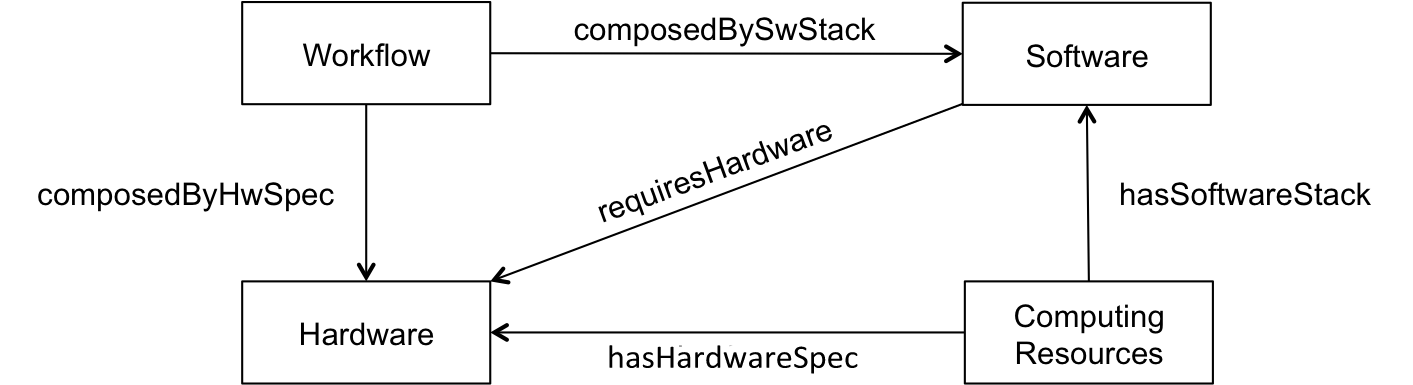
\includegraphics[width=.9\linewidth]{figures/wicusrels}
    \caption{Overview of the ontology network ($\rightarrow$ denotes inter-domain relation).}
    \label{fig:wicusrels}
\end{figure}

\section{Reproducibility in Scientific Workflows}
\label{sec:reproducibility}

In this section, we introduce the tools used in this work for the instantiation and evaluation 
of the semantic models aforementioned. We first describe the Pegasus Workflow 
Management System (WMS)~\cite{Pegasus, Deelman-FGCS-2014}, which is used as our 
workflow engine, and then a set of reproducibility tools for semantic annotations and 
experiment management.


\subsection{Scientific Workflow Execution}

The Pegasus WMS can manage workflows comprised of millions of tasks, recording data 
about the execution and intermediate results. In Pegasus, workflows are described as an 
abstract workflows, which do not contain resource information, or the physical locations of 
data and executables. Workflows are described as directed acyclic graphs (DAGs), where 
nodes represent individual computational tasks and the edges represent data and control 
dependencies between tasks. The abstract workflow description is represented as a DAX 
(DAG in XML), capturing all the tasks that perform computation, the execution order of these 
tasks, and for each task the required inputs, expected outputs, and the arguments with which 
the task should be invoked. 

During a workflow execution, Pegasus translates an abstract workflow into an 
executable workflow, determining the executables, data, and computational resources 
required for the execution. Pegasus maps executables to their installation paths or to a 
repository of stageable binaries defined in a Transformation Catalog (TC). A workflow 
execution includes data management, monitoring, and failure handling. Individual workflow 
tasks are managed by a task scheduler (HTCondor~\cite{condor}), which supervises their 
execution on local and remote resources.


\subsection{Reproducibility Tools}

To conduct the evaluation of the semantic models when executing scientific workflows, we 
use the WICUS framework~\cite{wicus}, which comprises the semantic models described 
in Section~\ref{sec:semantic} and a set of tools for annotating and consuming data; and 
the PRECIP~\cite{Azarnoosh-CRC-2013} experiment management tool to manage the 
experiment. In addition, we use Vagrant~\cite{palat2012introducing}, a tool for deploying virtual
deployment environments,  to achieve local reproducibility of the experiments. 
Below, we describe each of these tools in detail.


\subsubsection{WICUS}
We introduce here the Workflow Infrastructure Conservation Using Semantics ontology 
(WICUS), an OWL2~\cite{OWL2} (Web Ontology Language) ontology network that 
implements the semantic models introduced in Section~\ref{sec:semantic}. This ontology 
network is available online~\cite{wicus-online} and it is a continuous effort to discover and 
define the relevant and required properties for describing scientific computational infrastructures. 

Besides the ontology network, WICUS has a set of modules that facilitates the annotation of 
the resources involved on the execution of a scientific workflow. These tools are not fully 
automated yet, but represent a first step on helping users to define the requirements of their 
experiments. Figure~\ref{fig:wicusflow} shows the main modules, their flow and intermediate 
results involved in the process for achieving reproducibility, and describes the process of 
data generation and consumption. Below, we provide an overview of each of these modules:

\begin{figure}[!htb]
	\centering
	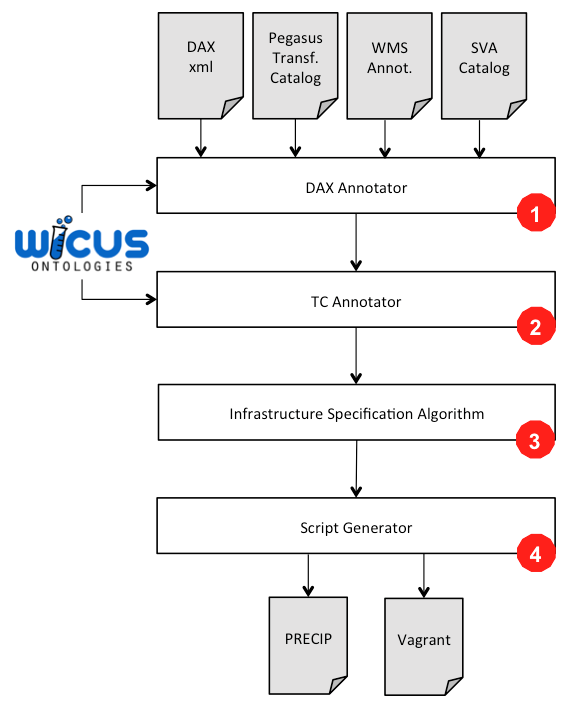
\includegraphics[width=.8\linewidth]{figures/wicusflow}
	\caption{WICUS annotation modules and flow. White boxes represent tools for semantic annotation or algorithms, and grey boxes represent files used or generated by the framework.}
	\label{fig:wicusflow}
\end{figure}

\begin{enumerate}
	\item \textbf{DAX Annotator.} This tool parses a DAX (Pegasus' workflow description) 
		and generates a set of annotations using the terms of the WICUS vocabulary, 
		representing workflow transformations and the workflow infrastructure requirements.

	\item \textbf{Workflow Annotations.} An RDF file containing the description of the workflow 
		and its infrastructure requirements.

	\item \textbf{WMS Annotations.} An RDF file containing the information of the WMS component 
		and its dependencies. This information will be added to the \emph{Software Components 
		Catalog}.

	\item \textbf{Transformation Catalog Annotator.} This tool parses the Pegasus Transformation 
		Catalog (which describes the binaries involved on the workflow execution and their locations) 
		and the WMS annotations file, to generate two set of annotations: the \emph{Software 
		Components Catalog} and the \emph{Workflow \& Configuration Annotation} files.

	\item \textbf{Software Components Catalog.} An RDF file containing the set of annotations about 
		the binaries, dependencies, deployment plans and scripts, and configuration information of 
		the software involved in the experiment.

	\item \textbf{Workflow \& Configuration Annotation File.} An RDF file containing the same information 
		as in 2, but enriched with the configuration information for each workflow execution step, as 
		specified in the transformation catalog.

	\item \textbf{Scientific Virtual Appliances Catalog.} An RDF file describing available VM appliances. 
		Information about the related infrastructure providers and the VM images that compose an 
		appliance are included in this dataset.

	\item \textbf{Infrastructure Specification Algorithm.} This process reads files 5, 6, and 7, and 
		generates a configuration file (e.g., a PRECIP script), which describes VMs and software 
		components to be created and deployed.

	\item \textbf{PRECIP script.} This script creates a PRECIP experiment, which runs a VM, copies 
		the required binaries, and executes deployment scripts to set the environment for the workflow 
		execution. It also contains the PRECIP commands from the original experiment in order to 
		re-execute it.

\end{enumerate}

In the experimental evaluation (Section~\ref{sec:experiment}), we will present a detailed description 
and the applicability of each module for the studied scientific workflows.



% PRECIP
\subsubsection{PRECIP}
The Pegasus Repeatable Experiments for the Cloud in Python (PRECIP)~\cite{Azarnoosh-CRC-2013} 
is a flexible experiment management control API for running experiments on all types of Clouds, 
including academic Clouds such as FutureGrid~\cite{futuregrid} and the NSFCloud~\cite{chameleon,cloudlab}, 
and commercial Clouds such as Amazon EC2~\cite{aws} and Google Compute Engine~\cite{gce}. 
In PRECIP, interactions with the provisioned instances are done by tagging. When an instance is 
provisioned, the scientist can add arbitrary tags to that instance in order to identify and group the 
instances in the experiment. API methods such as running remote commands, or copying files, all 
use tags to specify which instances to target. PRECIP does not force the scientist to use a special 
VM image, and no PRECIP components need to be pre-installed in the image. Scientists can use 
any basic Linux image and PRECIP will bootstrap instances using SCP and SSH commands. 
PRECIP provides functionality to run user-defined scripts on the instances to install/configure 
software and run experiments, and also manages SSH keys and security groups automatically.

In this work, PRECIP usage is twofold. First, the tool is used to describe and perform a workflow 
execution using the Pegasus WMS on a predefined VM image. Second, the WICUS annotation 
modules use PRECIP to generate a script able to reproduce the execution environment of the 
former experiment, and run it on different Cloud platforms.

\note{Should we add something about OpenStack@NSFCloud?}

% Vagrant
\subsubsection{Vagrant}

Vagrant~\cite{palat2012introducing} is an open-source and multi-platform solution for deploying 
development environments locally using virtualization. It relies on virtualization solutions such as 
Oracle VirtualBox~\cite{Watson2008} (also open-source) or  VMWare~\cite{vmware}, and support 
Amazon EC2-like server configurations. Since version 1.6 it also supports Docker~\cite{Merkel2014} containers.

Vagrant provides a set of commands and configuration files to enact and customize virtual machines
 (also referred as boxes). It allows to define the set of commands and/or scripts to be executed during 
 the different stages of the booting process. Several base images are publicly available for users to 
 download and customize them~\footnote{http://www.vagrantbox.es/}. 
 
 I this work we introduce how Vagrant can be used for achieving reproducibility at local environment, usually 
 on a scientist's laptop/desktop computer This brings access to users making it possible to repeat and modify 
 the original experiment, repurposing and/or improving it, which is a highly desirable goal of any reproducibility
 process.

%\note{Idafen to add some text about Vagrant.}


\section{Experimental Evaluation}
\label{sec:experiment}

The goal of this experiment is to reproduce original workflow executions in two different 
Cloud infrastructures: FutureGrid~\cite{futuregrid} and Amazon EC2~\cite{aws}. 
FutureGrid is an academic Cloud test-bed facility that includes a number of computational 
resources at distributed locations. Amazon Web Services EC2 is a public infrastructure 
provider and the \emph{de facto} standard for IaaS Cloud platforms.


\subsection{Scientific Workflows}

\paragraph{\textbf{Montage}}
The Montage workflow~\cite{Montage} was created by the NASA Infrared Processing 
and Analysis Center (IPAC) as an open source toolkit that can be used to generate 
custom mosaics of astronomical images in the Flexible Image Transport System (FITS) 
format. In a Montage workflow, the geometry of the output mosaic is calculated from the 
input images. The inputs are then re-projected to have the same spatial scale and rotation, 
the background emissions in the images are corrected to have a uniform level, and the 
re-projected, corrected images are co-added to form the output mosaic. 
Figure~\ref{fig:workflow-montage} illustrates a small (20 node) Montage workflow. The 
size of the workflow depends on the number of images required to construct the desired 
mosaic. The workflow instance used in this paper generate a 0.1 degree square mosaics 
using 15 input images from the 2 Micron All Sky Survey (2MASS).

\begin{figure}[!htt]
	\centering
	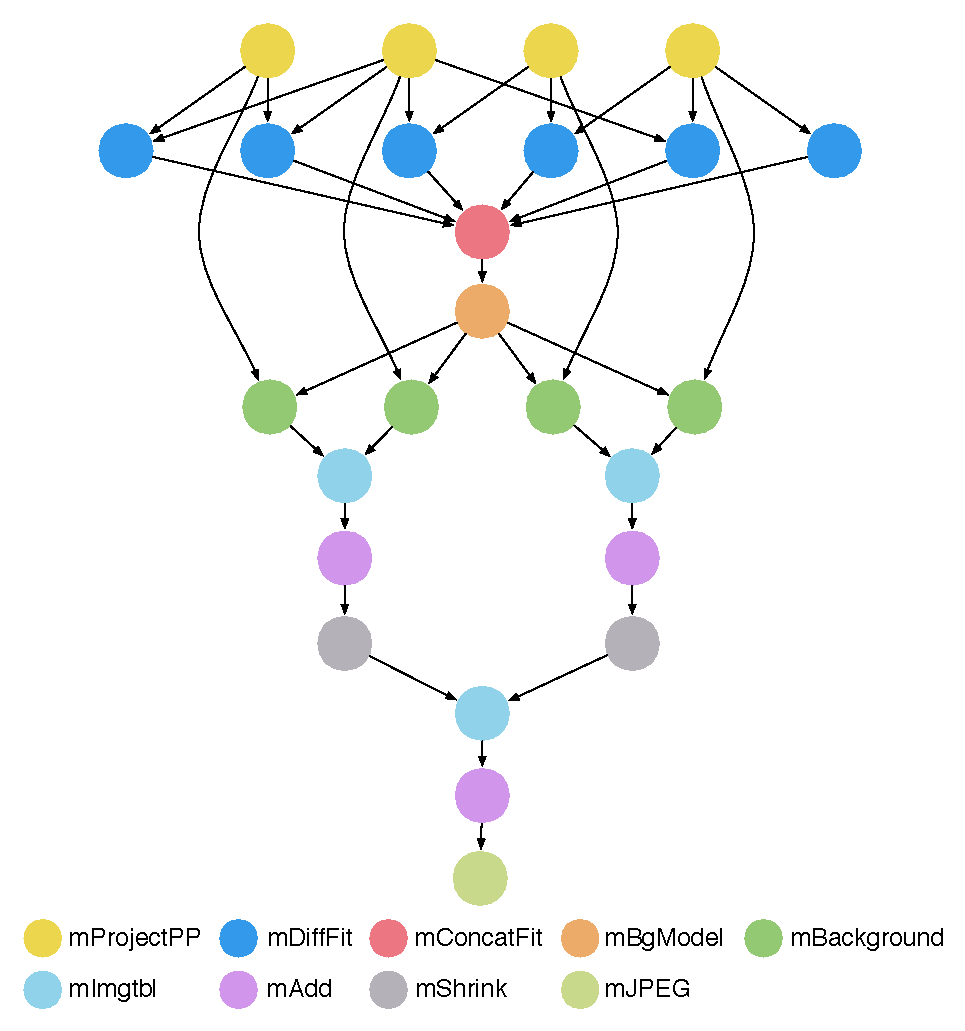
\includegraphics[width=0.9\linewidth]{figures/workflow-montage}
	\caption{A small (20 node) Montage workflow.}
	\label{fig:workflow-montage}
\end{figure}


\paragraph{\textbf{Epigenomics}}
The USC Epigenome Center~\cite{genome} is currently involved in mapping the epigenetic 
state of human cells on a genome-wide scale. The Epigenomics workflow 
(Figure~\ref{fig:workflow-genome}) processes multiple sets of genome sequences in
parallel. These sequences are split into subsets, the subsets are filtered to remove
contaminants, reformatted, then mapped to a reference genome. The mapped sequences are
finally merged and indexed for later analysis. In this work, the Epigenome workflow was 
used to align 13 million genome sequence reads to a reference genome for human 
chromosome 21. The size of the workflow depends on the chunking factor used on the input 
data (\texttt{binsize}), which determines the number of sequence reads in each chunk.

\begin{figure}[!htb]
	\centering
	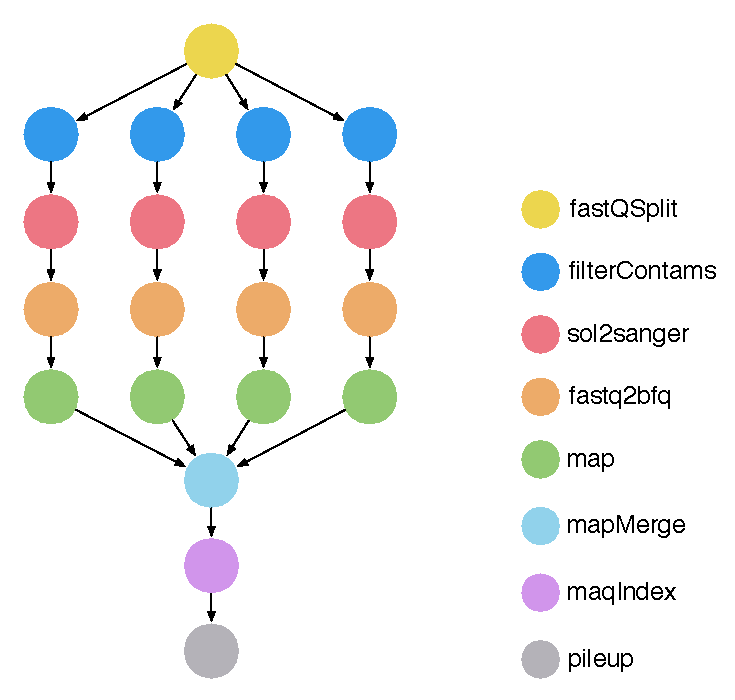
\includegraphics[width=0.75\linewidth]{figures/workflow-genome}
	\caption{Epigenomics workflow.}
	\label{fig:workflow-genome}
\end{figure}

\paragraph{\textbf{SoyKB}}
The SoyKB workflow~\cite{soybean, Joshi01012014} is a genomics pipeline 
that re-sequences soybean germplasm lines selected for desirable traits such 
as oil, protein, soybean cyst nematode resistance, stress resistance, and root 
system architecture. The workflow (Figure~\ref{fig:workflow-soykb}) 
implements a SNP and injection/deletion (indel) identification and analysis 
pipeline using the GATK haplotype caller~\cite{gatk} and a soybean reference 
genome. The workflow analyzes samples in parallel to align them to the reference 
genome, to de-duplicate the data, to identify indels and SNPs, and to merge and 
filter the results. The results are then used for genome-wide association studies 
(GWAS) and genotype to phenotype analysis. The workflow instance used in this 
paper is based on a sample dataset of 50 sequence reads that requires less 
memory than a full-scale production workflow.

\begin{figure}[!htb]
	\centering
	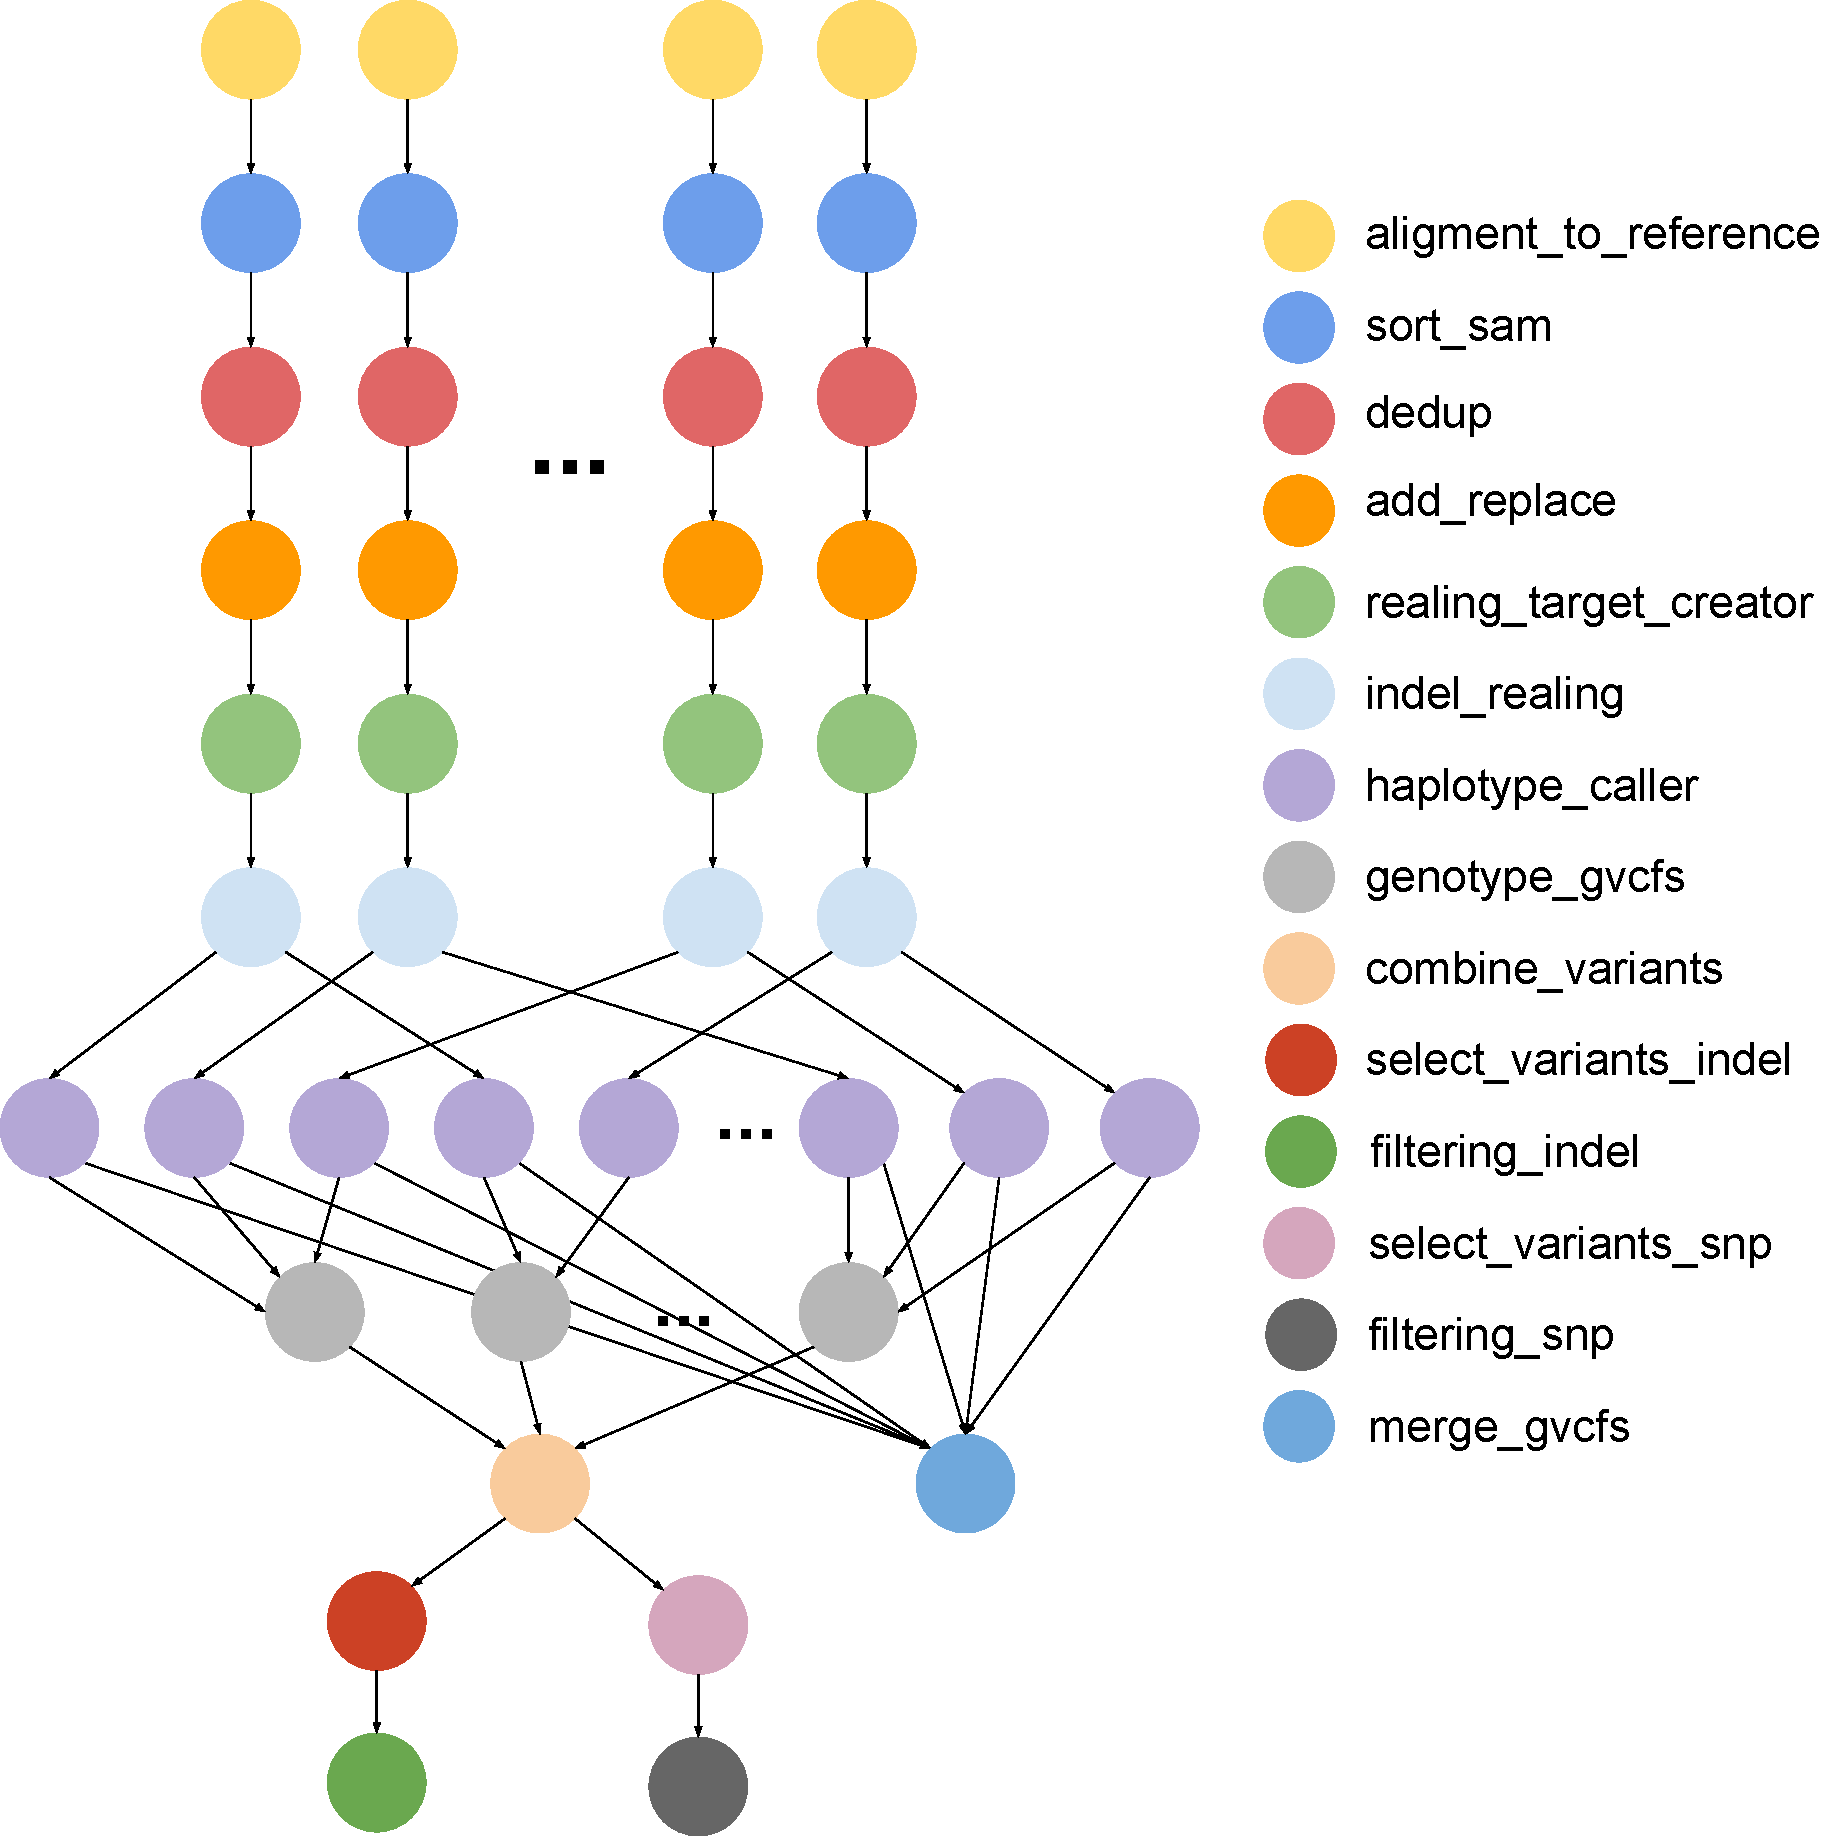
\includegraphics[width=0.95\linewidth]{figures/workflow-soybean}
	\caption{SoyKB workflow.}
	\label{fig:workflow-soykb}
\end{figure}


% Generating Semantic Annotations
\subsection{Generating Semantic Annotations}

\paragraph{\textbf{Montage}}
Figure~\ref{fig:annotations} shows a simplified overview of the annotations generated for the Montage workflow using the WICUS ontology network.

\begin{figure}[!htb]
	\centering
	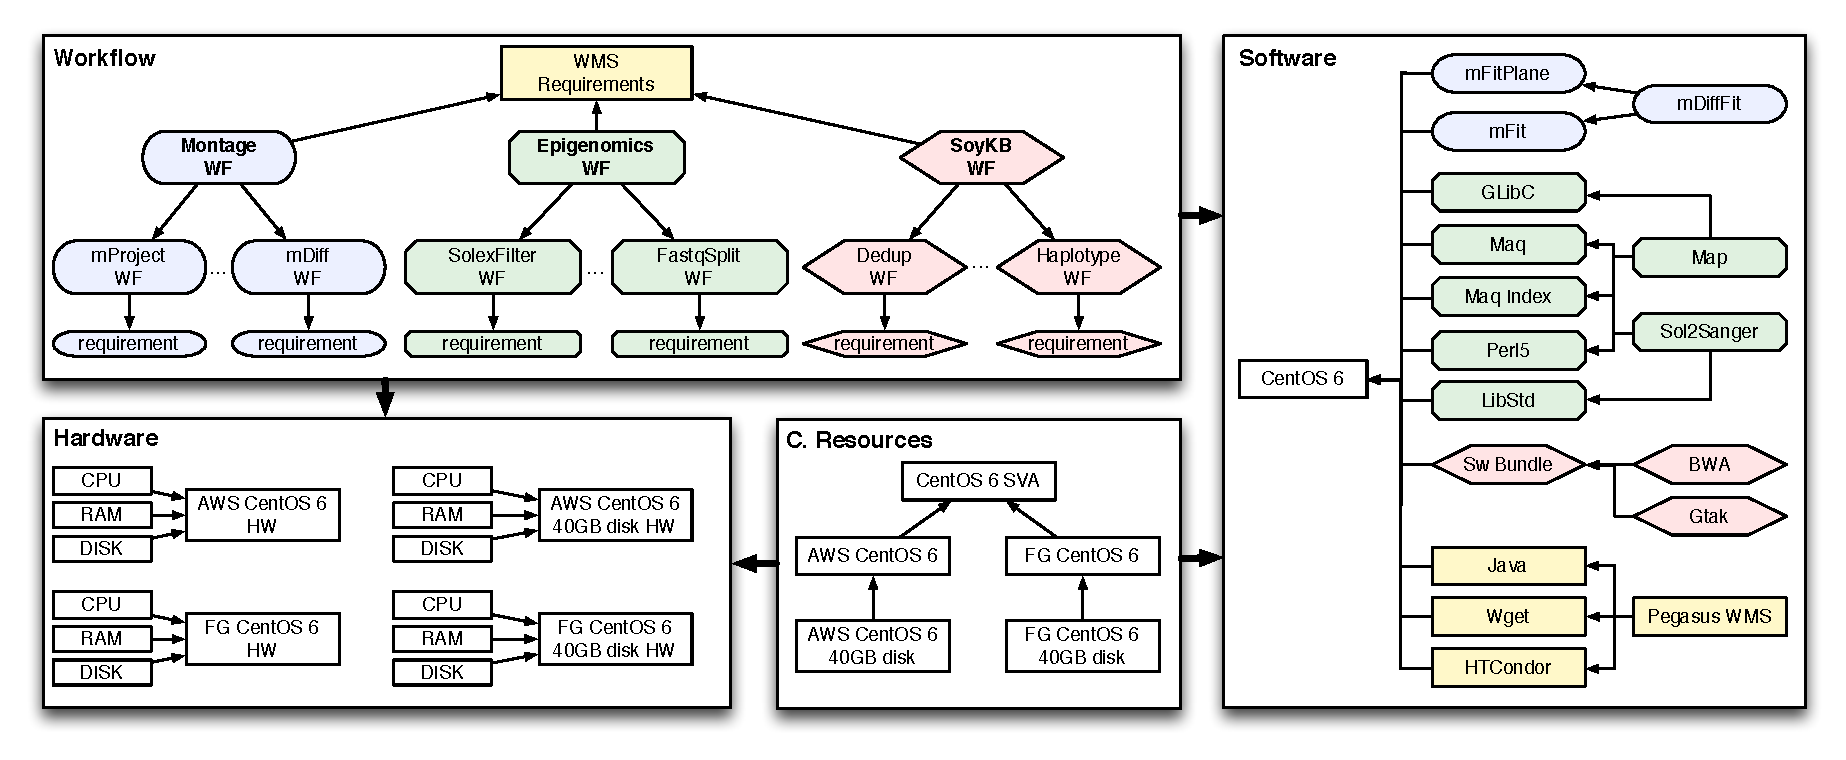
\includegraphics[width=\linewidth]{figures/annotations}
	\caption{Annotations for the Montage workflow using the WICUS ontology network.}
	\label{fig:annotations}
\end{figure}

As shown in Figure~\ref{fig:wicusflow}, the first step in the process of documenting a workflow is the annotation of the workflow DAX file. We use the \texttt{Workflow} domain ontology to describe the Montage workflow as 1) an individual that represents the top level workflow, and 2) another 9 individuals representing its sub-workflows, one for each transformation. We also generate 10 requirements, one for the top level workflow, which specifies the WMS requirements, and the remaining for defining the software components required by each transformation. At this point, these requirements are empty, as they are not yet related to their software components.
 
In this experiment, we address two types of components: the WMS and the application related components. The WMS components include the workflow engine, in our case the Pegasus WMS, and its dependencies. Pegasus uses HTCondor as task manager, and also depends on Java. We use the \texttt{Software} domain ontology to describe these components as individuals, and to represent their dependencies. The 3 components also depend on the operating system, which in our case is CentOS.

To describe the deployment of the WMS components, we studied their installation processes according to their documentation. We then defined a set of installation bash scripts for each of them. These scripts are included on the deployment plans of the components along with their configuration information.  
 
Application components are described from the Montage workflow's Transformation Catalog, where the binary file, version, and destination path are defined. These components are also described as individuals using the \texttt{Software} domain ontology. We use this information to generate the configuration parameters of the deployment script, which in this case is the same for all components. The script downloads the binary files from an online repository and copies them to the specified destination path. This process identified 59 software components for the Montage workflow that are annotated and included in the Software Components Catalog.
Then, the Transformation Catalog Annotator module relates each transformation requirement, defined using the \texttt{Workflow} domain ontology, to the application component, and therefore to the deployment information.
In this experiment, we define 9 Montage components that are linked to the requirements, and another two sub-components that are defined as dependencies in the software catalog (\emph{mDiffFit} depends on the \emph{mDiff} and \emph{mFitPlane} components).

To describe computational resources we use the \texttt{Computing Resources} and \texttt{Hardware} domain ontologies. The Scientific Virtual Appliances Catalog includes the description of two virtual machine images, one for FutureGrid and another for Amazon EC2. These two images are conceptually equivalent, as they both provide CentOS 6 operating system.
Therefore, we generate two Image Appliances (FG CentOS 6 and AWS CentOS 6) that are grouped into one single Scientific Virtual Appliance (CentOS 6 SVA). Depending on which providers are available, one or the other will be selected.


\subsection{Reproducing Workflow Executions.}

The last step on the process for achieving reproducibility in scientific workflows (Figure~\ref{fig:wicusflow}) is to execute the Infrastructure Specification Algorithm (ISA). The ISA combines the annotated data based on the 4 domain ontologies in order to find a suitable infrastructure specification that is able to run the workflow. The algorithm retrieves and propagates the WMS requirements of the top-level workflow (\texttt{Workflow} domain ontology) to its related sub-workflows. Requirements and software components are matched, and a dependency graph is built based on the relation between the requirements and the component dependencies. This graph is then used to compute the intersection between the set of software components from the SVA and the dependency graph of each sub-workflow. ISA selects the intersection where the value is maximized for each sub-workflow. Software components already available in the SVA are then removed from the chosen graph. To reduce the number of SVAs, the algorithm attempts to merge sub-workflows requirements into a single SVA. Requirements can be merged if all their software components are compatible. Finally, ISA generates a PRECIP script with the set of required instructions to instantiate, configure, and deploy the computational resources and software components.


In this experiment, we execute ISA over the annotated data in a scenario where FutureGrid is the only available platform for resource provisioning, and in a scenario where the available platform is Amazon EC2. In both cases, the algorithm is able to obtain a PRECIP script for each infrastructure. Each generated script is composed by the following main sections:

\begin{itemize}

	\item \emph{Experiment Creation}: generates a new experiment using the given VM image ID and the user credentials for the selected infrastructure provider;
    	    
	\item \emph{Software Deployment}: executes the set of instructions defined on the deployment plan of each software component to install and configure the required software to execute the workflow. In this section, both the workflow management system and the application are deployed with their dependencies;

	\item \emph{User Setup}: creates a user account on the VM (if it does not exist) and configures the necessary SSH keys to enable file transfers and execution. This account will be used to run the workflow;
	   
	\item \emph{Data Stage and Workflow Execution}: stages all the input data of the Montage workflow on the VM, and launches the workflow execution. Since our work is focused on infrastructure reproducibility, data and workflow management are not covered in our approach.

\end{itemize}

\noindent Note that all the configuration and deployment commands (first 3 sections) require superuser privileges on the VM. The workflow execution, however, is performed under the user account created in the third section.

We executed the scripts on their corresponding platforms. Both executions succeeded on deploying and running the Montage workflow, the Pegasus WMS, and their dependencies. We also performed the same execution of the Montage workflow in a predefined VM image, where the execution environment is already in place. Results show that the VM execution environments deployed by both scripts are equivalent to the former one. In addition, we used a perceptual hash tool\footnote{pHash - \url{http://www.phash.org}} to compare the resulting image (0.1 degree image of the sky) generated by both executions against the one generated by the baseline execution. We obtained a similarity factor of 1.0 (over 1.0) with a threshold of 0.85, which means the images are identical. Therefore we are obtaining the same results as the original workflow. In this work we do not aim to reproduce either the performance or the execution time of the original experiment.


All the original and generated scripts are available as part of the experimental material included in the Research Object (RO)~\cite{researchObjects} associated with this paper\footnote{\url{http://pegasus.isi.edu/publications/reppar}}. This RO also contains pointers to the software and resources used in this experiment.
\section{Related Work}
\label{sec:related-work}

A computational experiment involves several elements that must be conserved 
to ensure reproducibility. In the last year several studies and initiatives have been 
conducted for solving its associated challenges~\cite{Hothorn01052011,Sylwester14}. 
Most of the works address the conservation of data and the workflow description, 
however the computational environment is often neglected. Recent studies have 
exposed the necessity of publishing adequate descriptions of the runtime environment of experiments to avoid replication hindering~\cite{Rollins201459}. As a result, there is an increase on the number of publications 
providing associated experimental materials~\cite{Brown2012, diginorm}.

A study to evaluate reproducibility in scientific workflows is conducted in~\cite{zhao2012}. The study evaluates a set of domain-specific workflows, available in  myExperiment~\cite{myExperiment}, to identify causes of workflow decay. The study shows that nearly 80\% of the workflows cannot be reproduced, that about 12\% of these reproducibility issues are due to the lack of information about the execution environment, and that 50\% of them are due to the use of third-party resources such as web services and databases that are not available anymore. Note that some of those third-party resource issues could be also considered as execution environment problems, as many of them are remote services for information processing. 

Recently, another comprehensive study has been published~\cite{Collberg2015}, surveying 601 papers from ACM conferences and studying how authors share the data and code supporting their results. Authors found that 402 of those papers were supported by code. In this study authors tried to obtain the code related to each publication, looking for links within the paper itself, searching on code repositories, and contacting the authors when necessary. After the code was obtained, several students were asked to try to build it. This whole process was limited by experimental design to a period of 30 minutes. Results show that in 32.3\% of the 402 papers students were able to obtain the code and build the code within the given period. In 48.3\% of the cases, code was built with some extra effort, and in 54\% of the papers code was either built or the authors stated the code would build with reasonable effort. Authors propose, as a result of this study, a {\it sharing specification} for publications that allow to state the level of sharing of each paper.

The workflow paradigm has been widely adopted in the bioinformatics community, for studying genome sequencing ~\cite{blankenberg2010galaxy, giardine2005galaxy, kepler-clotho}, disease-related experiments~\cite{fisher2009systematic, gaizauskas2004} and many others. Several studies have exposed the difficulties of trying to reproduce experimental results on life sciences, such as biology~\cite{Ioannidis2009}. and cancer analysis~\cite{ErringtonCancerRerpoducibility}.

Replicability and reproducibility of computational experiments using cloud computing resources and software descriptions have been widely proposed as an approach for those studies in which performance is not a key experimental result~\cite{Crick14}.

The Executable Paper Grand Challenge~\cite{elsevierchallenge} and the SIGMOD conference in 2011~\cite{SIGMOD} highlighted the importance of allowing the scientific community to reexamine experiment execution. The conservation of virtual machine (VM) images emerges as a way of preserving the execution environment~\cite{Brammer,SHARE}. However, the high storage demand of VM images remains a challenging problem~\cite{Mao:2014:ROD:2600090.2512348,6552826}. Moreover, the cost of storing and managing data in the Cloud is still high, and the execution of high-interactivity experiments through a network connection to remote virtual machines is also challenging. A list of advantages and challenges of using VMs for achieving reproducibility is exposed in~\cite{Howe2012}. ReproZip~\cite{reprozip} is a provenance-based tool that tracks operating system calls to identify the libraries and data dependencies, as well as the configuration parameters involved in an experiment. The tool combines all these dependencies into a single package that can be used to reproduce an experiment. Although this approach avoids storing VM images, it still requires storing the application binaries and their dependencies. Instead, our work uses semantic annotations to describe these dependencies.

%\feedback{@Maria: add more references to previous work on life science reproducibility}
%\note{Idafen: there are several references to this in the introduction. Should we repeat them here?}

Galaxy~\cite{goecks2010galaxy}, a well know workflow system in the context of life sciences, proposes a web-service based system for achieving accessible and reproducible computations. Galaxy hides the implementation details of the underlying tools for workflow developers, providing a web-based interface for retrieving an analyzing genomic data. Even when this approach has proved to be successful in several cases, we argue that it does not cover local development of workflows, which is a common case on computational science.  


Software components cannot be preserved just by maintaining their binary executable code, but by guaranteeing the performance of their features. In~\cite{Matthews}, the concept of adequacy is introduced to measure how a software component behaves relatively to a certain set of features. Our work is based on this same concept, where we build a conceptual model to semantically annotate the relevant properties of each software component. Then, we use scripting to reconstruct an equivalent computational environment using these annotations.

A recent and relevant contribution to the state of the art of workflow preservation has been developed within the context of the TIMBUS project~\cite{Mayer2014Ontologies}. The project  aimed to preserve and ensure the availability of business processes and their computational infrastructure, aligned with the enterprise risk and the business continuity managements. They also proposed a semantic approach for describing the execution environment of a process.  However, even though TIMBUS has studied the applicability of their approach to the eScience domain, their approach is mainly focused on business processes.

Semantics have been also proposed in the area of biomedical research as a way for achieving reproducibility of published experiments~\cite{MaloneSWO2014}. In this work authors propose to annotate the software artifacts in the same way that gene products or phenotypes are annotated. In order to do so, authors propose the {\it Software Ontology} (SWO), a model for describing the software involved on the storage and management of data. The SWO have many concepts in common with the WICUS ontology  network, but is specialized on the biomedical domain, focusing on modeling biomedical-related software specifically. WICUS aims to be a more generic ontology that can be applied in different scientific domains.


\section{Conclusion and Future Work}
\label{sec:conclusion}

In this work, we proposed a semantic modeling approach to conserve 
computational environments in scientific workflow executions, where  
the resources involved in the execution of the experiment are described 
using a set of semantic vocabularies. We defined and implemented four 
domain ontologies, aggregated in the the WICUS ontology network. From 
these models, we defined a process for documenting workflow applications, 
the workflow management system, and their dependencies.

We conducted experiments with three real workflow applications (Montage, 
Epigenomics, and SoyKB) from different sciences using the Pegasus WMS. 
We used the Infrastructure Specification Algorithm (ISA) to obtain a set of 
PRECIP and Vagrant scripts to describe and execute the experiment. 
Experimental results show that our approach can reproduce an equivalent 
execution environment of a predefined VM image on academic, public, and 
local Cloud platforms.

Semantic annotations of the computational environment, combined with the 
ISA and the scripting functionality provided by PRECIP and Vagrant, is a 
powerful approach for achieving reproducibility of computational environments 
in future experiments, and at the same time addresses the challenges of high 
storage demand of VM images. \rev{In this work, we have demonstrated that
an equivalent computational environment (that fulfills the requirements of a
workflow) can be obtained from simple base VM images, which are already 
available in most Cloud platforms. Consequently, there is no need to create 
and store a new VM image for each workflow. Therefore, this approach 
significantly diminishes the costs and efforts in maintaining a VM image that 
may have limited usage. We acknowledge that this approach may be limited 
to the online (publicly) availability of the software, however most of the scientific
tools developed nowadays are hosted as an open-source project.}

% how by using a generic VM image, only containing the operating system and its default associated tools, we have been able to dynamically generate three different virtual machines, each of them fulfilling the requirements of a workflow. These images are public and were already available and supported by the different providers we have worked with. Thus, we have saved several gigabytes by not generating an image for each workflow.}
%\note{Not sure how to quantify the amount of GB we save. We could ask Mats for the size of the WM Images at FG, but not sure how to calculate the size of the AWS and Vagrant VMs}

%\rev{This kind of solution requires the workflow management system and the scientific applications related to the workflow to be publicly available. We argue that this necessary condition holds in most cases, being the majority of software solutions developed in science open and public}. 

\rev{To attain reproducibility, the proposed model requires that information about
the software components involved on the workflow execution should be available
and as explicit as possible. In Pegasus, the transformation catalog provides 
all necessary information. Similar catalogs (or files) are also available in other
workflow systems. }
%\rev{For achieving the reproducibility of the workflow execution environment, as we have done in this work, access to the resources describing the workflow is required. The information about the software components involved on the execution must be available and as explicit as possible. In the case of the experiments of this work, the Pegasus Transformation Catalog file provided this information, which is also available in other workflow systems using similar files.}
\rev{Also, knowledge about semantic technologies is required for generating 
some of the annotations for describing the underlying infrastructure. Currently,
the description of the WMS and the computational resources are manually 
generated, whereas the remaining annotations are performed by tools of the 
WICUS system. Future work include the development of tools to fully (or 
partially) automate this process. The annotation process may be assisted 
by experts, in the same way librarians aid book authors and publishers to 
conserve their contributions.}
%Nevertheless, as those annotations are reused, we argue that this effort is reasonable.

The results of this work also show how components, such as the workflow 
system, can be annotated once and then reused among workflows. We 
envision a library of workflow descriptions in which components and tools 
can be easily reused, even during the development process of the workflow. 
Many workflows are built upon previous workflows, especially within the 
context of a scientific domain, and hence having such type of library would 
be helpful. We plan to study how and when those libraries can be built, 
analyzing their degree of reuse. \rev{As introduced in this work, our 
descriptions of the environment, generated using the WICUS ontology 
network, is compliant with the Linked Data principles. This would allow its 
future publication and integration with other information sources, which fits 
the idea of a distributed and structured library of descriptions that could be 
publicly available worldwide.}

\rev{We are currently studying the applicability of our approach to other 
workflow applications (from different scientific areas) and systems. Although
the Cloud systems included in this work cover a representative spectrum of 
Cloud providers, we are also considering other Cloud scenarios and 
emerging container-based solutions. Also, we plan to extend the scope of 
our approach to enable reproducibility of more complex and larger execution 
infrastructures, such as multi-node clusters and topology-specific network 
platforms.}
% New cloud management systems and enactment files will be also explored in the future, aiming to evaluate their performance and suitability according to the goals of our work.}
% We will study how our approach can reproduce those characteristics.

We will also work on increasing  the degree of automation of the semantic annotation process to describe both the workflow application and the workflow management system. As introduced in this work, WICUS is an ongoing effort, thus we also plan to extend the ontology network to include new concepts and relations such as software variants, incompatibilities, and user policies for resource consumption.







% Acknowledgements
\section*{Acknowledgements}

This material is based upon work supported in part by the National Science Foundation under Grant No. 0910812 to Indiana University for ``FutureGrid: An Experimental, High-Performance Grid Test-bed'' and the FPU grant from the Spanish Science and Innovation Ministry (MICINN). We also thank Gideon Juve and Karan Vahi for their valuable help.


% Bibliography
\bibliographystyle{elsarticle-num}
\bibliography{references}

\end{document}